\subsubsection{Octrees}

\begin{frame}
\frametitle{Octrees --- What is an octree?}
\begin{columns}[c]

\column{.5\textwidth}

\begin{itemize}[<+(1)->]
\item A tree data structure
\item Each node corresponds to a physical cube
\item The child nodes represents cubes half the size of their parent's
\item Each node has place for eight child nodes
\end{itemize}

\column{.45\textwidth}
\begin{figure}
\centering
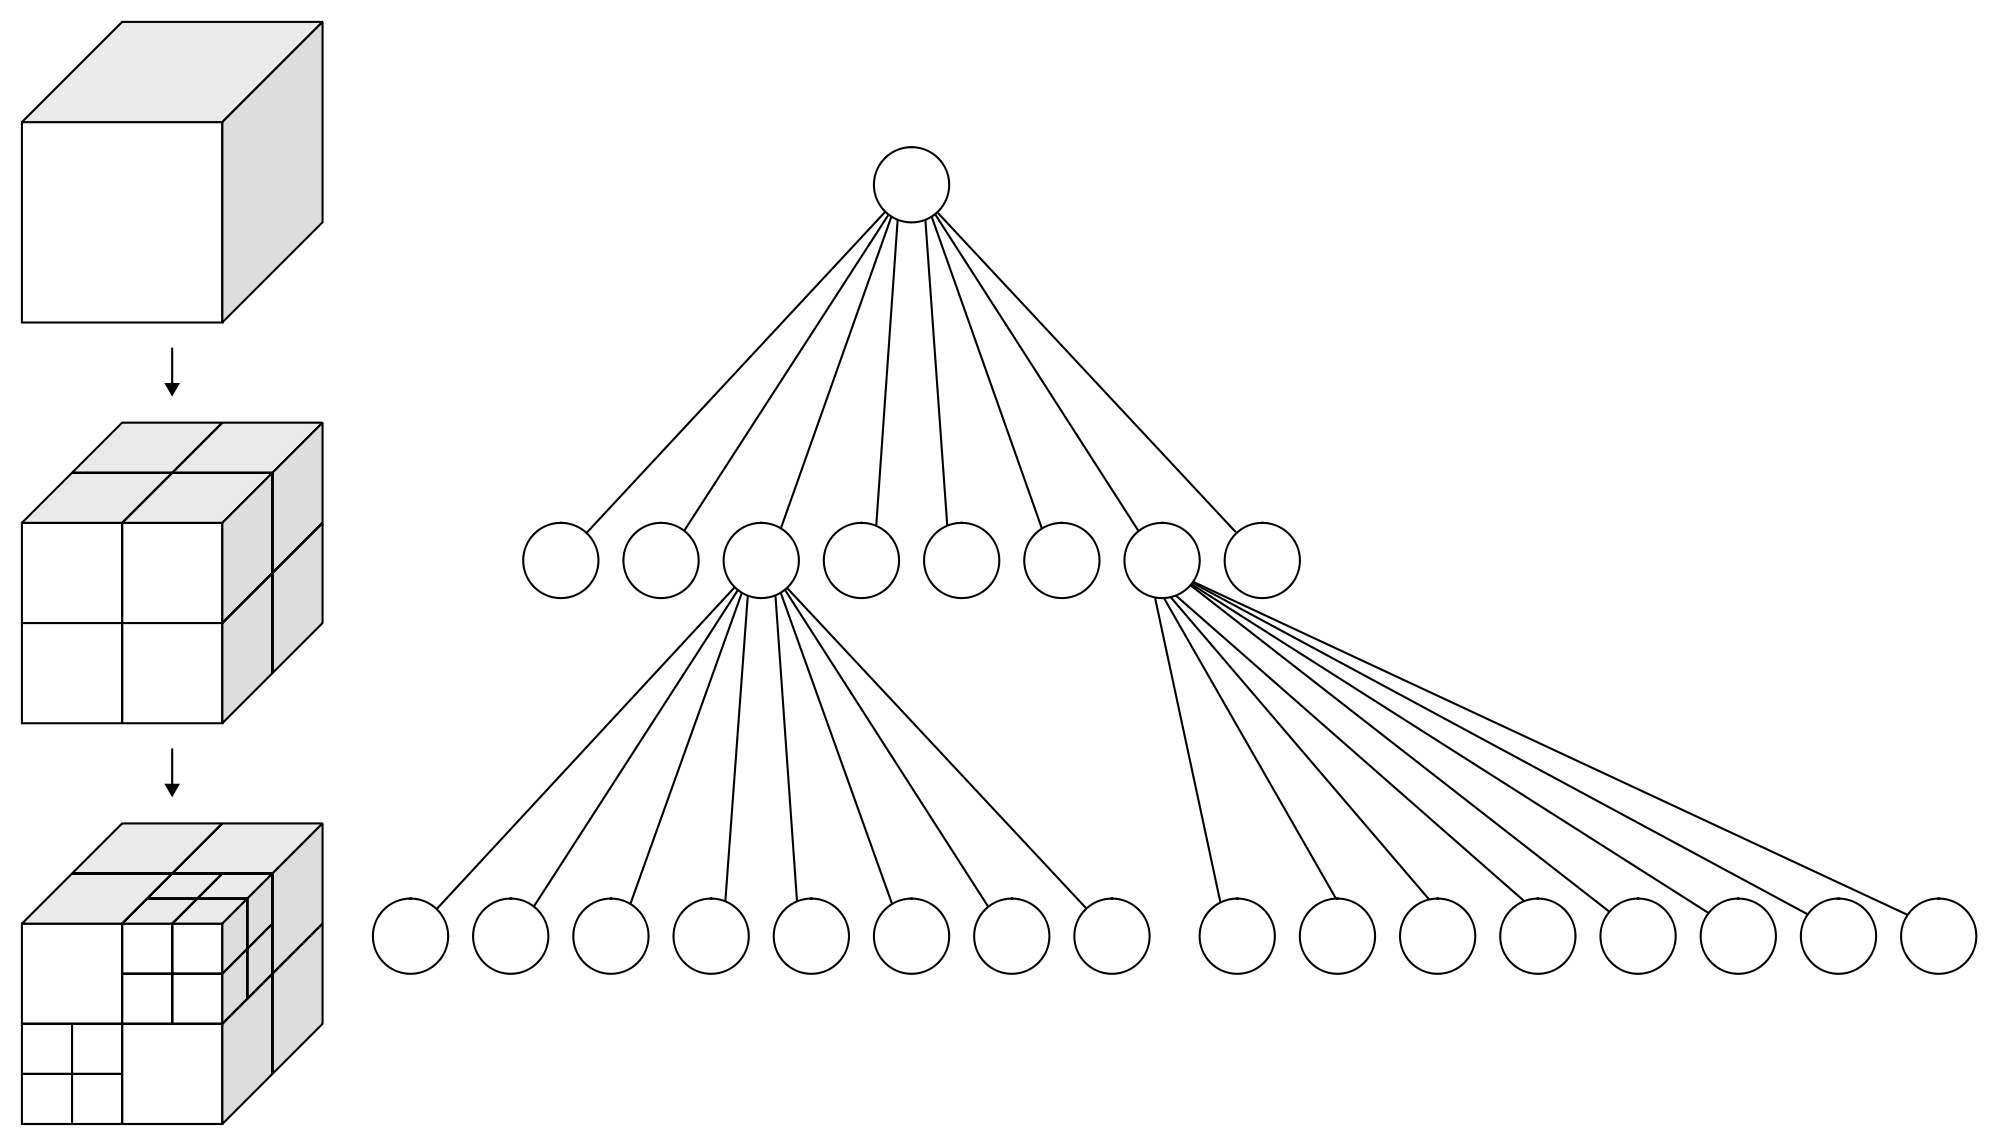
\includegraphics[width=\textwidth]{Images/Attribute/Octree/2000px_Octree2_svg}
\caption{Retrieved from http://commons.wikimedia.org/\allowbreak wiki/\allowbreak File:Octree2.svg}
%\end{figure}
%\begin{figure}
    \centering
    %\subcaptionbox{\label{fig:quadtree}}[\textwidth]{
        \begin{tikzpicture}[x={(.3\textwidth,0)},y={(0,.3\textwidth)}]
            % Front side
            \draw (0,0,1) \threedimsquarepath{1} {1}{0}{0} {0}{1}{0};
            % Level 1
            \drawthreedimplus{0}{0}{1} {1} {1}{0}{0} {0}{1}{0}
            % Level 2
            \drawthreedimplus{1/2}{1/2}{1} {1/2} {1}{0}{0} {0}{1}{0}
            \drawthreedimplus{1/2}{0/2}{1} {1/2} {1}{0}{0} {0}{1}{0}
            \drawthreedimplus{0/2}{1/2}{1} {1/2} {1}{0}{0} {0}{1}{0}
            % Level 3
            \drawthreedimplus{2/4}{3/4}{1} {1/4} {1}{0}{0} {0}{1}{0}
            \drawthreedimplus{3/4}{3/4}{1} {1/4} {1}{0}{0} {0}{1}{0}
            \drawthreedimplus{2/4}{1/4}{1} {1/4} {1}{0}{0} {0}{1}{0}
            % Level 4
            \drawthreedimplus{5/8}{7/8}{1} {1/8} {1}{0}{0} {0}{1}{0}
            \drawthreedimplus{6/8}{7/8}{1} {1/8} {1}{0}{0} {0}{1}{0}
            \drawthreedimplus{5/8}{6/8}{1} {1/8} {1}{0}{0} {0}{1}{0}
            \drawthreedimplus{6/8}{6/8}{1} {1/8} {1}{0}{0} {0}{1}{0}
            % Level 5
            \drawthreedimplus{12/16}{14/16}{1} {1/16} {1}{0}{0} {0}{1}{0}
            \drawthreedimplus{11/16}{14/16}{1} {1/16} {1}{0}{0} {0}{1}{0}
            \drawthreedimplus{11/16}{13/16}{1} {1/16} {1}{0}{0} {0}{1}{0}
            \drawthreedimplus{10/16}{13/16}{1} {1/16} {1}{0}{0} {0}{1}{0}
        \end{tikzpicture}
    %}
    \quad
    %\vskip 1em
    %\subcaptionbox{\label{fig:octree}}[\textwidth]{
        \begin{tikzpicture}[x={(.3\textwidth,0)},y={(0,.3\textwidth)},z={(-.385*.3\textwidth,-.385*.3\textwidth)}]
            % Front side
            \draw[fill=white!100!black] (0,0,1) \threedimsquarepath{1} {1}{0}{0} {0}{1}{0};
            % Level 1
            \drawthreedimplus{0}{0}{1} {1} {1}{0}{0} {0}{1}{0}
            % Level 2
            \drawthreedimplus{1/2}{1/2}{1} {1/2} {1}{0}{0} {0}{1}{0}
            \drawthreedimplus{1/2}{0/2}{1} {1/2} {1}{0}{0} {0}{1}{0}
            \drawthreedimplus{0/2}{1/2}{1} {1/2} {1}{0}{0} {0}{1}{0}
            % Level 3
            \drawthreedimplus{2/4}{3/4}{1} {1/4} {1}{0}{0} {0}{1}{0}
            \drawthreedimplus{3/4}{3/4}{1} {1/4} {1}{0}{0} {0}{1}{0}
            \drawthreedimplus{2/4}{1/4}{1} {1/4} {1}{0}{0} {0}{1}{0}
            % Level 4
            \drawthreedimplus{5/8}{7/8}{1} {1/8} {1}{0}{0} {0}{1}{0}
            \drawthreedimplus{6/8}{7/8}{1} {1/8} {1}{0}{0} {0}{1}{0}
            \drawthreedimplus{5/8}{6/8}{1} {1/8} {1}{0}{0} {0}{1}{0}
            \drawthreedimplus{6/8}{6/8}{1} {1/8} {1}{0}{0} {0}{1}{0}
            % Level 5
            \drawthreedimplus{12/16}{14/16}{1} {1/16} {1}{0}{0} {0}{1}{0}
            \drawthreedimplus{11/16}{14/16}{1} {1/16} {1}{0}{0} {0}{1}{0}
            \drawthreedimplus{11/16}{13/16}{1} {1/16} {1}{0}{0} {0}{1}{0}
            \drawthreedimplus{10/16}{13/16}{1} {1/16} {1}{0}{0} {0}{1}{0}
            %
            % Top side
            \draw[fill=white!98!black] (0,1,0) \threedimsquarepath{1} {1}{0}{0} {0}{0}{1};
            % Level 1
            \drawthreedimplus{0}{1}{0} {1} {1}{0}{0} {0}{0}{1}
            % Level 2
            \drawthreedimplus{0/2}{1}{1/2} {1/2} {1}{0}{0} {0}{0}{1}
            \drawthreedimplus{1/2}{1}{1/2} {1/2} {1}{0}{0} {0}{0}{1}
            \drawthreedimplus{1/2}{1}{0/2} {1/2} {1}{0}{0} {0}{0}{1}
            % Level 3
            \drawthreedimplus{2/4}{1}{3/4} {1/4} {1}{0}{0} {0}{0}{1}
            \drawthreedimplus{3/4}{1}{3/4} {1/4} {1}{0}{0} {0}{0}{1}
            \drawthreedimplus{2/4}{1}{2/4} {1/4} {1}{0}{0} {0}{0}{1}
            % Level 4
            \drawthreedimplus{5/8}{1}{7/8} {1/8} {1}{0}{0} {0}{0}{1}
            \drawthreedimplus{6/8}{1}{7/8} {1/8} {1}{0}{0} {0}{0}{1}
            \drawthreedimplus{5/8}{1}{5/8} {1/8} {1}{0}{0} {0}{0}{1}
            %
            % Right side
            \draw[fill=white!90!black] (1,0,0) \threedimsquarepath{1} {0}{1}{0} {0}{0}{1};
            % Level 1
            \drawthreedimplus{1}{0}{0} {1} {0}{1}{0} {0}{0}{1}
            % Level 2
            \drawthreedimplus{1}{1/2}{1/2} {1/2} {0}{1}{0} {0}{0}{1}
            \drawthreedimplus{1}{0/2}{1/2} {1/2} {0}{1}{0} {0}{0}{1}
            \drawthreedimplus{1}{1/2}{0/2} {1/2} {0}{1}{0} {0}{0}{1}
            \drawthreedimplus{1}{0/2}{0/2} {1/2} {0}{1}{0} {0}{0}{1}
            % Level 3
            \drawthreedimplus{1}{3/4}{3/4} {1/4} {0}{1}{0} {0}{0}{1}
            \drawthreedimplus{1}{2/4}{2/4} {1/4} {0}{1}{0} {0}{0}{1}
            \drawthreedimplus{1}{2/4}{1/4} {1/4} {0}{1}{0} {0}{0}{1}
            \drawthreedimplus{1}{1/4}{2/4} {1/4} {0}{1}{0} {0}{0}{1}
            \drawthreedimplus{1}{1/4}{1/4} {1/4} {0}{1}{0} {0}{0}{1}
            % Level 4
            \drawthreedimplus{1}{3/8}{3/8} {1/8} {0}{1}{0} {0}{0}{1}
            \drawthreedimplus{1}{4/8}{3/8} {1/8} {0}{1}{0} {0}{0}{1}
            \drawthreedimplus{1}{4/8}{4/8} {1/8} {0}{1}{0} {0}{0}{1}
        \end{tikzpicture}
    %}
    \caption{Source: Own}
    \label{fig:quadtree_and_octree}
\end{figure}

\end{columns}
\end{frame}


\begin{frame}
\frametitle{Octrees --- Pros/Cons}
%\begin{columns}[c]

%\column{.6\textwidth}

\begin{itemize}[<+(1)->]
\proitem \emph{Pro}: Adaptive grid refinement (necessity!)
\conitem \emph{Con}: Unstructured grid
\end{itemize}


%\column{.5\textwidth}

\begin{figure}
\centering
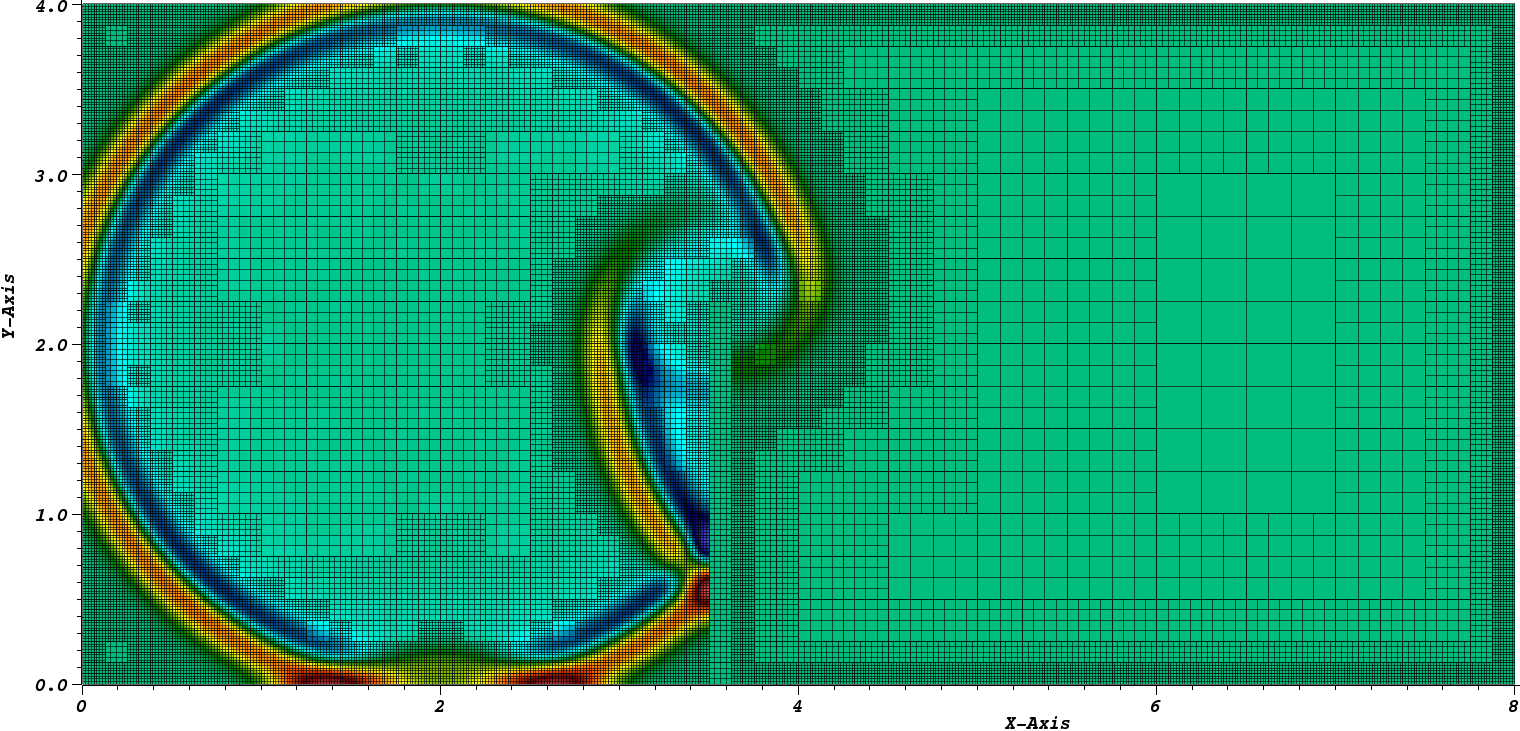
\includegraphics[width=\textwidth]{Images/Attribute/AMR/Amr}
\caption{Retrieved from http://commons.wikimedia.org/\allowbreak wiki/File:Amr.png}
\end{figure}

%\end{columns}
\end{frame}
